Increase the usability and viability of cloud resources for scientific applications.

Resource and cost management, automation. Abstractions. 

Middleware. HPC as a service.


This paper combines and integrates instance selection, fault-tolerance policies, and application-specific policies.

Prior approaches have largely explored each of these facets individually, and running scientific workloads in the cloud has not received the attention that it warrants.

We show that costs in the cloud can be reduced by up to $10\times$ with the combination of smart server selection, preemption aware resource allocation, and ``job-importance'' thresholds for job-groups.

Explicit E[Recomputation Time] equation. 


No angle brackets

Assumptions

P() = min(1,)

We generate bags of jobs by changing so so and so parameter.

Established long-term cross disciplanry collaborations here. 

Alibaba Cloud Spot Instances 
https://www.alibabacloud.com/help/doc-detail/52088.htm

Packet Bare Metal Cloud Spot Market
https://support.packet.com/kb/articles/spot-market

The preemptions of transient servers need not be related to their price.
-For example, Google's Preemptible VMs and Azure Batch VMs have a \emph{fixed} price relative to their non-preemptible counterparts. 
-In such cases, price-based models are inadequate, and other approaches to understand preemptions are required.
 
-This task is further complicated by the fact that these cloud operators (Google and Microsoft) do not currently provide any information about preemption characteristics. 
-Thus, relatively little is known about the preemptions (and hence the performance) of these transient VMs. %significantly limiting their use?
-%
-To understand preemption dynamics of transient servers, we conduct a large-scale empirical measurement study. 
 We launched more than 1,500 Google Preemptible VMs of different types over a two month period (Feb--April 2019), and measured their time to preemption (i.e., their useful lifetime).\footnotemark
 
 \footnotetext{We will release the complete preemption dataset for further analysis.} %Weaksauce 
 
 
 \begin{figure}
-  \centering
-  \includegraphics[width=0.4\textwidth]{../graphs/scispot-fig-cdf-prob-inset-time.eps}
-  \vspace*{-0.2cm}
-  \caption{CDF of lifetimes of Google Preemptible VMs. Our proposed distribution for modeling the constrained preemption dynamics provides better fits to the empirical data compared to the conventional exponential and the Weibull distributions. Inset shows the probability of failure as a function of time for the three distributions.}
-  \vspace*{\captionspace}
-


-To describe failures (preemptions) that are not memoryless (i.e., increasing or decreasing failure rate over time), the classic Weibull distribution with CDF $F(t)=1-e^{-(\lambda t)^k}$ is often employed. However, the Weibull distribution is also unable to fit the empirical data (Figure~\ref{fig:gcp1}). 
-
-The non-trivial bathtub-shaped failure rate of Google preemptible VMs (Figure~\ref{fig:gcp1}) requires models that capture the sudden onset of  the rise in preemptions near the deadline. 
-%which imposes a dynamics that is more akin to a constrained dynamics problem as opposed to dynamics characterized with a gradually rising failure rate.
-Our new model, informed by the cumulative distribution of lifetimes that has multiple distinct temporal phases, addresses this need. The key assumption underlying our model is the presence of two distinct failure processes.

-% Since cloud platforms support a wide range of applications, they also offer a large range of servers (VMs) with different resource configurations (such as the number of CPU cores, memory size, I/O bandwidths, etc.). 
-% For example, a cloud provider may offer VMs with (4 CPUs, 4 GB memory), (8 CPUs, 8 GB memory), etc.
-% Most clouds offer a large number of different hardware configurations---Amazon EC2 offers more than 50 hardware configurations, for example~\cite{amazon-ec2-instance-types}.



In this section, we present empirical and analytical evaluation of the performance and cost of \sysname with different scientific computing workloads and scales. 
Our evaluation consists of empirical analysis, as well as model-driven simulations for analyzing and comparing \sysname behavior under different preemption and application dynamics.

We shed insight into the fundamental tradeoffs in constrained preemptions, the effectiveness of our model-based policies, and detailed empirical analysis of the cost and performance of our \sysname framework with real-world scientific computing applications. 
We have already established the goodness of fit of our model and compared it to existing models earlier in Section~\ref{sec:failmodel}. 

% \begin{itemize}
% \item What is performance and cost of 
% \end{itemize}
All applications use OpenMPI v2.1.1, are deployed on Slurm v0.4.3 and 64-bit Ubuntu 18.04, and run on Google Cloud VMs with x86-64 Intel Haswell CPUs. 
% Networking?
For completeness and to guard against concerns about poor cloud performance relative to HPC clusters ~\cite{iosup_performance_2011, zhai_cloud_2011, marathe2013comparative, galante_analysis_2016, benedictis_cloud-aware_2014}, we benchmarked the Nanoconfinement application on the Big Red II cluster~\cite{bigred2}. 
When run on 4 nodes with 16 CPUs each, the application takes 1140 seconds on Big Red II vs 850 seconds on \sysname. 
We attribute the 20\% improvement with \sysname to the newer CPUs on Google Cloud (Intel Haswell vs. older 2012-era AMD Opterons in Big Red II).

%For completeness, we show the running times on the Big Red II supercomputing cluster in Table~\ref{tab:bigred2}, with 16 CPU nodes used throughout, and we see that our representative applications \emph{do not} face a penalty when deployed on the cloud. 

\vspace*{\subsecspace}

%%% Local Variables:
%%% mode: latex
%%% TeX-master: "paper"
%%% End:
